%----------------------------------------------------------------------------
\chapter{Jegyzőkönyv}
%----------------------------------------------------------------------------
%----------------------------------------------------------------------------
\section{Első feladat}
%----------------------------------------------------------------------------
PyTorch segítségével definiáltunk egy \textit{Conv} osztályt, mely a 2D konvolúción kívül tartalmaz még \textit{BatchNorm} réteget és \textit{ReLU} aktivációt is. A hálót definiáló \textit{ConvNet} osztály pedig erre építve állítottuk össze, 6 \textit{Conv} és egy \textit{nn.Linear} rétegből áll, ez utóbbi szolgáltatja az egyes osztályokhoz tartozó kimeneteket.
%----------------------------------------------------------------------------
\section{Második feladat}
%----------------------------------------------------------------------------
A CIFAR adatbázis része a PyTorch \textit{torchvision} moduljának, így néhány parancs segítségével betöltöttük. Adatdúsításhoz véletlen képrészlet kivágást, vízszintes tükrözést és színtér transzformációkat alkalmaztunk, ezen kívül minden minta előkészítésénél szükség volt PyTorch tenzorrá alakításra és normalizációra. Az előbb említett funkciókat és a batchek előkészítését a \textit{transforms} modul és a DataLoader osztály végezte.
A következő hiperparaméterek hatásával kísérleteztünk a különböző tanítások során:

\begin{itemize}
	\item \textbf{Planes} - az egyes Conv blokkok 2D konvolúciós rétegeinek számát határozza meg.
	\item \textbf{LR} - learning rate, egy tanítási lépés során a gradienst ezzel skálázzuk le.
	\item \textbf{Momentum} - Az újonnan számolt gradiens aránya, ehhez az előző gradienseket is hozzáadjuk súlyozva, így megakadályozhatjuk a lokális minimumba ragadást.
	\item \textbf{Weight Decay} - arány L2 loss számolásához, a súlyok növekedését akadályozza meg.
	\item \textbf{Batch Size} - egy tanítási lépés alatt a háló egyszerre ennyi adat alapján számít gradienst.
\end{itemize}

\newpage
%----------------------------------------------------------------------------
\subsection{Első futás}
%----------------------------------------------------------------------------
\begin{table}[h]
	\begin{tabular}{|l|l|l|l|l|}
		\hline
		\textbf{Planes} & \textbf{LR} & \textbf{Momentum} & \textbf{Weight Decay} & \textbf{Batch Size} \\
		8 & 0.1 & 0.9 & 0.0001 & 128 \\ \hline
		\textbf{Futási idő} & \textbf{Training Acc.} & \textbf{Training Loss} & \textbf{Valid. Acc.} & \textbf{Valid. Loss} \\
		6m 43s & 73.44 & 0.7793 & 75.87 & 0.6925 \\ \hline
	\end{tabular}
	\caption{Az első futás eredménye}
\end{table}
Az első tanítást tekinthetjük viszonyítási alapnak.

%----------------------------------------------------------------------------
\subsection{Második futás}
%----------------------------------------------------------------------------
\begin{table}[h]
	\begin{tabular}{|l|l|l|l|l|}
		\hline
		\textbf{Planes} & \textbf{LR} & \textbf{Momentum} & \textbf{Weight Decay} & \textbf{Batch Size} \\
		8 & \textit{0.01} & 0.9 & 0.0001 & 128 \\ \hline
		\textbf{Futási idő} & \textbf{Training Acc.} & \textbf{Training Loss} & \textbf{Valid. Acc.} & \textbf{Valid. Loss} \\
		6m 44s & 71.38 & 0.8304 & 74.21 & 0.7389 \\ \hline
	\end{tabular}
	\caption{A második futás eredménye}
\end{table}
A második tanítás során csökkentettük a learning rate-et. Az eredmény rosszabb lett, így már túl lassan tanult a háló. 10 epochonként automatikus LR csökkentést alkalmaztunk, ez amúgy is hamar kis LR-t eredményez, érdemes a tanítást nagy értékkel kezdeni.


%----------------------------------------------------------------------------
\subsection{Harmadik futás}
%----------------------------------------------------------------------------
\begin{table}[h]
	\begin{tabular}{|l|l|l|l|l|}
		\hline
		\textbf{Planes} & \textbf{LR} & \textbf{Momentum} & \textbf{Weight Decay} & \textbf{Batch Size} \\
		8 & 0.1 & \textit{0} & 0.0001 & 128 \\ \hline
		\textbf{Futási idő} & \textbf{Training Acc.} & \textbf{Training Loss} & \textbf{Valid. Acc.} & \textbf{Valid. Loss} \\
		6m 52s & 70.07 & 0.8657 & 72.60 & 0.7699 \\ \hline
	\end{tabular}
	\caption{A harmadik futás eredménye}
\end{table}
A harmadik tanítás momentum nélkül futott. Jelen esetben is csökkent a háló teljesítménye, hiszen a lokális minimumok könnyebben befolyásolták, téves irányokba terelték a gradienst.




%----------------------------------------------------------------------------
\subsection{Negyedik futás}
%----------------------------------------------------------------------------
\begin{table}[h]
	\begin{tabular}{|l|l|l|l|l|}
		\hline
		\textbf{Planes} & \textbf{LR} & \textbf{Momentum} & \textbf{Weight Decay} & \textbf{Batch Size} \\
		8 & 0.1 & 0.9 & 0.0001 & \textit{32} \\ \hline
		\textbf{Futási idő} & \textbf{Training Acc.} & \textbf{Training Loss} & \textbf{Valid. Acc.} & \textbf{Valid. Loss} \\
		10m 3s & 70.10 & 0.8657 & 73.67 & 0.7533 \\ \hline
	\end{tabular}
	\caption{A negyedik futás eredménye}
\end{table}
Ebben az esetben kevesebb minta tartozott egy batch-be. Így jóval több tanítási ciklusra volt szükség, hogy epoch-onként az összes mintát felhasználjuk. A python mátrix kezelő könyvtárai jól optimalizáltan dolgoznak, nagyobb mátrixok helyett több ciklust használni sebesség csökkenést okoz. Ezen kívül a teljesítmény is romlott, a kisebb batchekkel kevésbé általánosan jó irányokba haladt a háló.

\newpage
%----------------------------------------------------------------------------
\subsection{Ötödik futás}
%----------------------------------------------------------------------------
\begin{table}[h]
	\begin{tabular}{|l|l|l|l|l|}
		\hline
		\textbf{Planes} & \textbf{LR} & \textbf{Momentum} & \textbf{Weight Decay} & \textbf{Batch Size} \\
		\textit{16} & 0.1 & 0.9 & 0.0001 & 128 \\ \hline
		\textbf{Futási idő} & \textbf{Training Acc.} & \textbf{Training Loss} & \textbf{Valid. Acc.} & \textbf{Valid. Loss} \\
		7m 6s & 79.90 & 0.6010 & 81.35 & 0.5379 \\ \hline
	\end{tabular}
	\caption{Az ötödik futás eredménye}
\end{table}
Az 5. tanításnál megdupláztuk a háló rétegeinek számát. A több súly miatt lassabban teljesítette a program a 20 epochot, cserébe jelentős teljesítmény növekedést értünk el, bonyolultabb összefüggések tanulására lett képes a háló. 


%----------------------------------------------------------------------------
\subsection{Hatodik futás}
%----------------------------------------------------------------------------
\begin{table}[h]
	\begin{tabular}{|l|l|l|l|l|}
		\hline
		\textbf{Planes} & \textbf{LR} & \textbf{Momentum} & \textbf{Weight Decay} & \textbf{Batch Size} \\
		\textit{16} & 0.1 & 0.9 & \textit{0} & 128 \\ \hline
		\textbf{Futási idő} & \textbf{Training Acc.} & \textbf{Training Loss} & \textbf{Valid. Acc.} & \textbf{Valid. Loss} \\
		7m 7s & 80.22 & ? & 81.56 & 0.5432 \\ \hline
	\end{tabular}
	\caption{A hatodik futás eredménye}
\end{table}
Az előző esethez hasonlóan maradt a teljesítmény és futási idő növekedés. A súlyokból számolt költség elhagyása nem hozott jelentős változást.

\newpage
%----------------------------------------------------------------------------
\subsection{Összegzés}
%----------------------------------------------------------------------------
A \figref{Train}~ és a \figref{Val}~ábrákon láthatóak a különböző futások eredményei összesített grafikonok. 
\begin{figure}[!h]
	\centering
	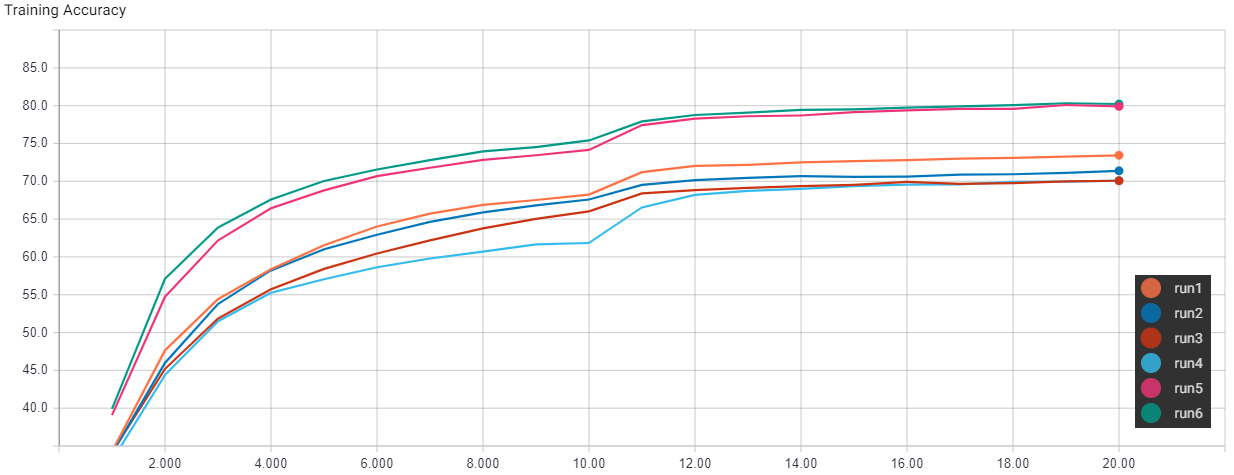
\includegraphics[width=125mm, keepaspectratio]{figures/m07/train_acc2.jpg}\\\vspace{2mm}
	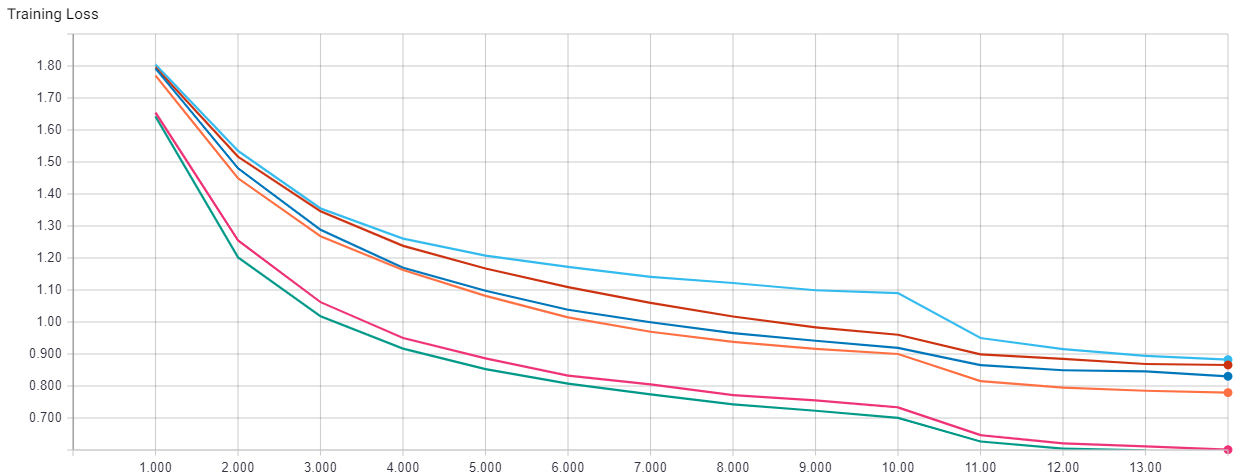
\includegraphics[width=125mm, keepaspectratio]{figures/m07/train_loss.jpg}
	\caption{Tanítási eredmények}
	\label{fig:Train}
\end{figure}
\begin{figure}[!h]
	\centering
	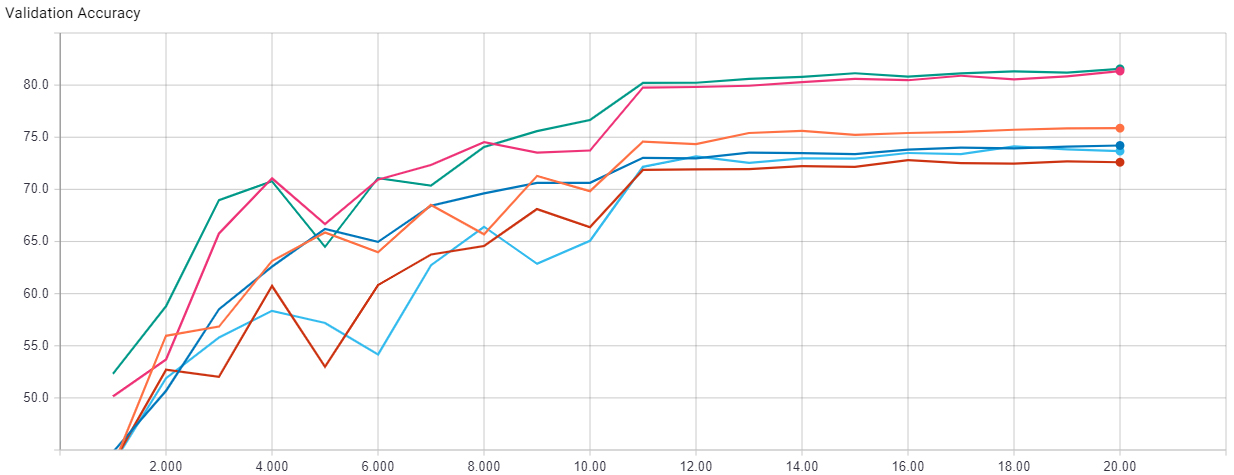
\includegraphics[width=125mm, keepaspectratio]{figures/m07/val_acc.jpg}\\\vspace{2mm}
	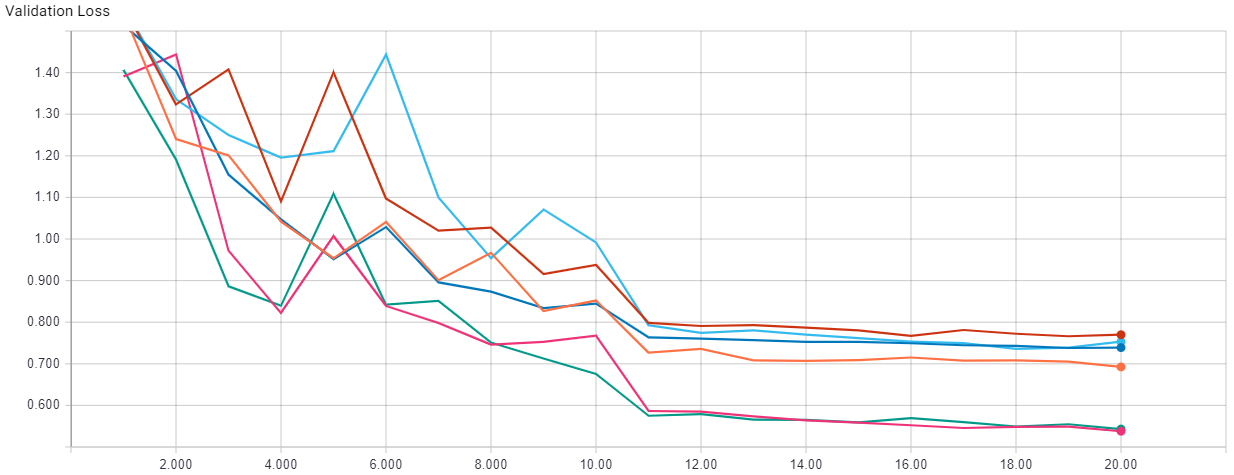
\includegraphics[width=125mm, keepaspectratio]{figures/m07/val_loss.jpg}
	\caption{Validálási eredmények}
	\label{fig:Val}
\end{figure}

\newpage
\newpage

%----------------------------------------------------------------------------
\section{Harmadik feladat}
%----------------------------------------------------------------------------
A DenseNet tanításához az eredeti hiperparaméter kombinációt (\textit{Learning Rate}=0.1, \textit{Momentum}=0.9, \textit{Weight Decay}=0.0001, \textit{Batch Size}=128) választottuk, ezek mellett, csak az epochok számát (100-ra) és a \textit{LearningRate Scheduler} paramétét (25 epochra) változtattuk. Az előző feladatokban használt általunk megírt modell helyett, a mérésvezető által kijelölt DenseNet struktárára állítottuk a tanítandó modellt. Az így módosított fájlokat az egyetem DeepLearning szerverére feltöltöttük, majd SSH segítségével egy terminál ablakban elindítottuk a tanítást. Mivel a tanítás hosszabb ideig tartott, mint a laboratórium, így az eredményeket az egyetem honlapján megjelenő TensorBoard segítségével utólagosan tudtuk kiértékelni.

A grafikonok a vártnak megfelelő működést mutatnak, a haló kb 50 epoch után beszaturált, a tanítási pontosság elérte a 99\%-ot. A validációs pontosság 93\% körül tetőzött, e kettő érték aránya mutatja, hogy a DenseNet struktúrája és a benne lévő batch normalizációs rétegek is jól működtek, a jóval mélyebb háló ellenére is sikerült elkerülni a túlillesztés jelenségét.

A tanítási hiba grafikonján látni, hogy megfelelő tanítási rátát választottunk, a tanítás elején a konvergencia erős, ám konstans gyengül. Az első ütemezett tanítási ráta csökkentése (25. epoch) után ugrásszerűen növekszik, majd a ismét legyengül. A második csökkentés (50. epoch után) hatása még látható a grafikonon, de ezután érdemi változást nem lehet látni, a hiba szinte 0-ba konvergált.

\begin{figure}[!h]
	\centering
	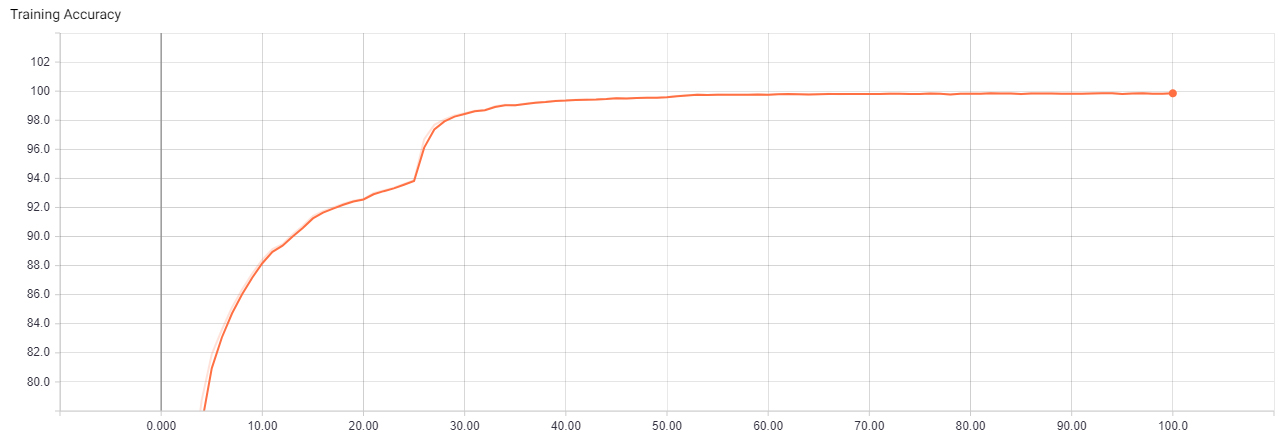
\includegraphics[width=140mm, keepaspectratio]{figures/m07/dn_train_acc.jpg}\\\vspace{5mm}
	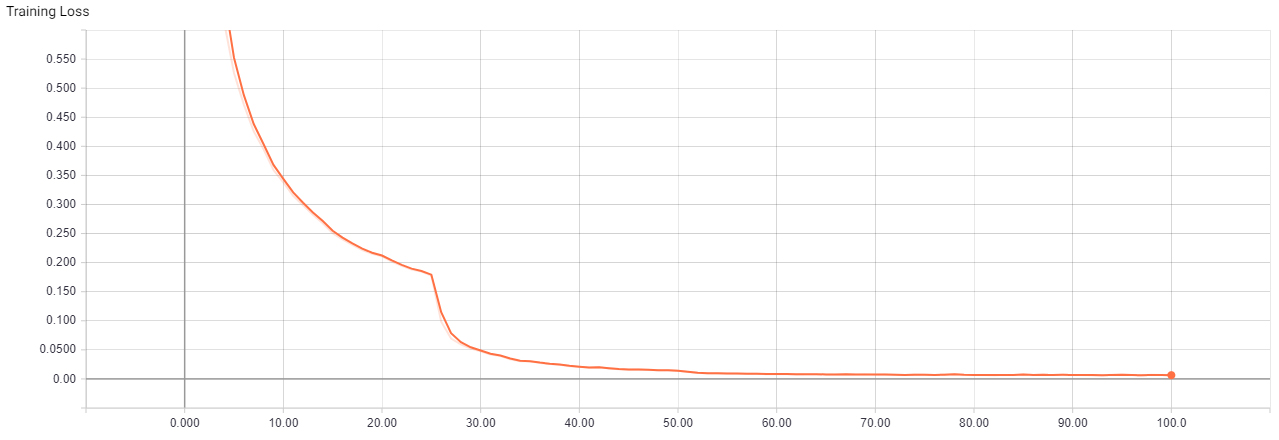
\includegraphics[width=140mm, keepaspectratio]{figures/m07/dn_train_loss.jpg}
	\caption{Tanítási eredmények a DenseNet struktúrán}
	\label{fig:TrainDense}
\end{figure}
%----------------------------------------------------------------------------
\section{Negyedik feladat}
%----------------------------------------------------------------------------
A feladathoz egy előre tanított AlexNet modellt használtunk, mely a PyTorch-ból egyszerűen betölthető. Első lépésként a korábbi feladatokkal megegyezően a kamera képét bemenetként adtuk a hálónak, majd a legbiztosabbra becsült kimenetet ‘1’ értékűnek véve a \textit{GuidedBckprop} osztály segítségével gradienseket generáltunk a háló bemenetére.
A gradiensek abszolútértékeit pixelenként szummáztuk, majd küszöbözés és legnagyobb kontúr keresés után bejelölhetővé vált a képen az a régió, amely a háló döntését leginkább befolyásolta.
Sok esetben a háló nem a prediktált objektum, hanem annak környezete alapján döntött. Például gyakran szerepelt “csokornyakkendő” vagy “öltöny” címke, amikor embereket látott a kamera, vagy “falióra” címke egy üres falat nézve. Ennek oka, hogy a tévesztett és valódi objektumok szorosan együtt járnak, a tanításhoz használt képeken mindig szerepel ember a csokornyakkendővel együtt, vagy üres falfelületen látható a falióra.



\begin{figure}[!h]
	\centering
	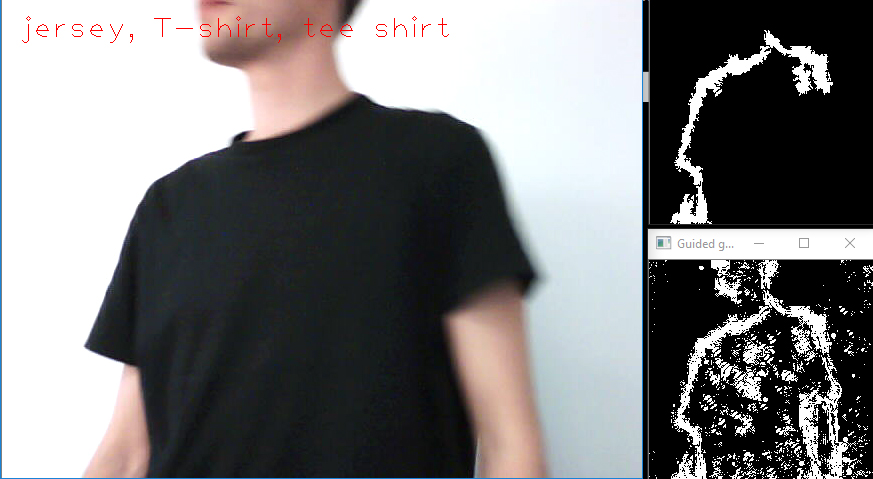
\includegraphics[width=69mm, keepaspectratio]{figures/m07/Untitled-.jpg}\hspace{5mm}
	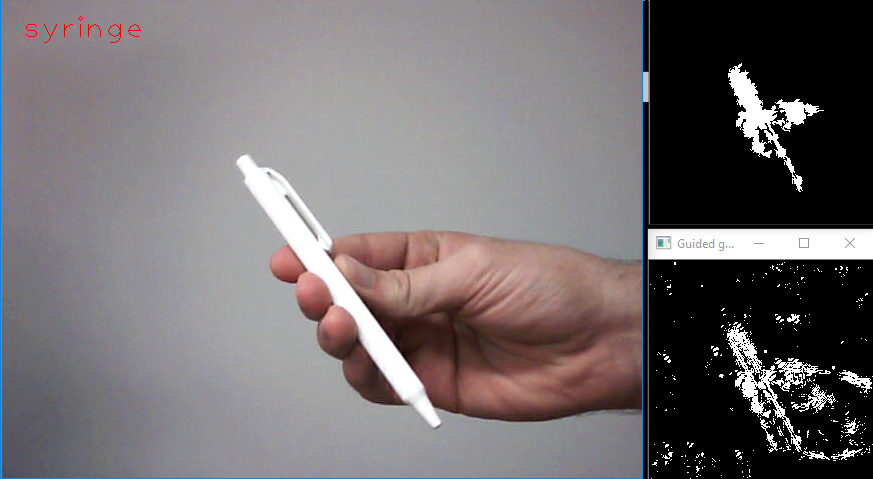
\includegraphics[width=69mm, keepaspectratio]{figures/m07/Untitled-2.jpg}\\\vspace{5mm}
	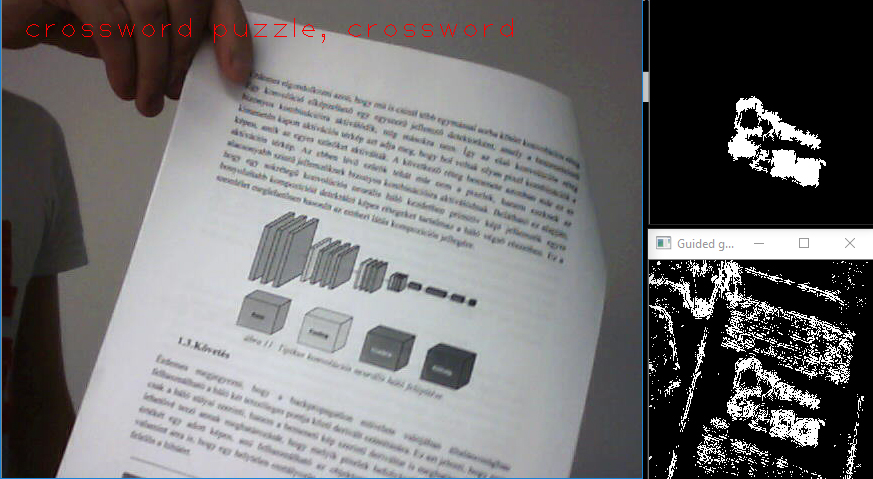
\includegraphics[width=69mm, keepaspectratio]{figures/m07/Untitled-3.jpg}\hspace{5mm}
	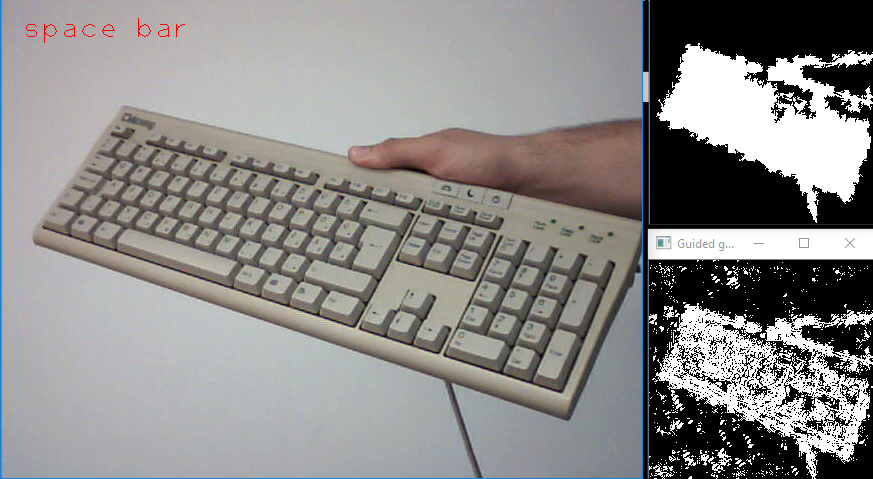
\includegraphics[width=69mm, keepaspectratio]{figures/m07/Untitled-4.jpg}
	\caption{A Guided Propagation megvalósítása különböző objektumokra}
	\label{fig:poi}
\end{figure}





































